\documentclass{article}
\usepackage[T1]{fontenc}
\usepackage{kpfonts}
\usepackage{amssymb}
\usepackage{listings}
\usepackage[utf8x]{inputenc}
\usepackage{amsmath,amssymb}
\usepackage{pdfpages}
\usepackage[russian,english]{babel}
\lstset{
    language=Octave,
    frame=single,
    inputencoding=utf8x,
    extendedchars=\true,
    texcl=\false,
    breaklines=true,
    breakatwhitespace=true,
    commentstyle={}
}
\usepackage[a4paper,top=1cm,bottom=2cm,left=1.5cm,right=1cm,marginparwidth=1.75cm]{geometry}

\makeatletter
\def\@seccntformat#1{
  \expandafter\ifx\csname c@#1\endcsname\c@section\else
  \csname the#1\endcsname\quad
  \fi}
\makeatother

\begin{document}

\selectlanguage{russian}
\title{ТВМС, Лабораторная работа 8, Вариант 10}
\author{
	Ковешников Глеб, M3238\\
	kovg16@gmail.com
}
\maketitle

\begin{quote}
\selectlanguage{russian}
\section{Формулировка}
\subsection{Задание 1}
  \begin{itemize}
    \item Смоделировать квадратичную функцию, наблюдаемую в нормальных шумах в соответствии с заданными параметрами.
    \item Оценить коэффициенты квадратичной зависимости, уровень шумов и квадратичную функцию по зашумленным данным.
    \item Сравнить результаты с исходными данными.
  \end{itemize}
\subsection{Задание 2}
  \begin{itemize}
    \item Смоделировать линейную функцию, наблюдаемую в нормальных шумах в соответствии с заданными параметрами.
    \item Оценить коэффициенты линейной зависимости, уровень шумов и линейную функцию по зашумленным данным.
    \item Построить доверительный интервал для значений функции при уровне доверия $0.95$.
    \item Сравнить результаты с исходными данными.
  \end{itemize}
\section{Входные данные}
  \begin{itemize}
    \item Границы интервала: $x_{min} = 1.3, x_{max} = 2.5$
    \item Число точек: $n = 60$
    \item Коэффициенты квадратичной функции: $a_1 = 2.2, a_2 = -3.2, a_3 = 4.5$
    \item Коэффициенты линейной функции: $c_1 = 2.2, c_2 = 1.5$
    \item Уровень шумов: $s = 3.7$
  \end{itemize}
\section{Исходный код}
\subsection{Квадратичная функция}
  \lstinputlisting{task1.txt}
\subsection{Линейная функция}
  \lstinputlisting{task2.txt}
\section{Результат работы программ}
\subsection{Квадратичная функция}
  \lstinputlisting{out1.txt}
  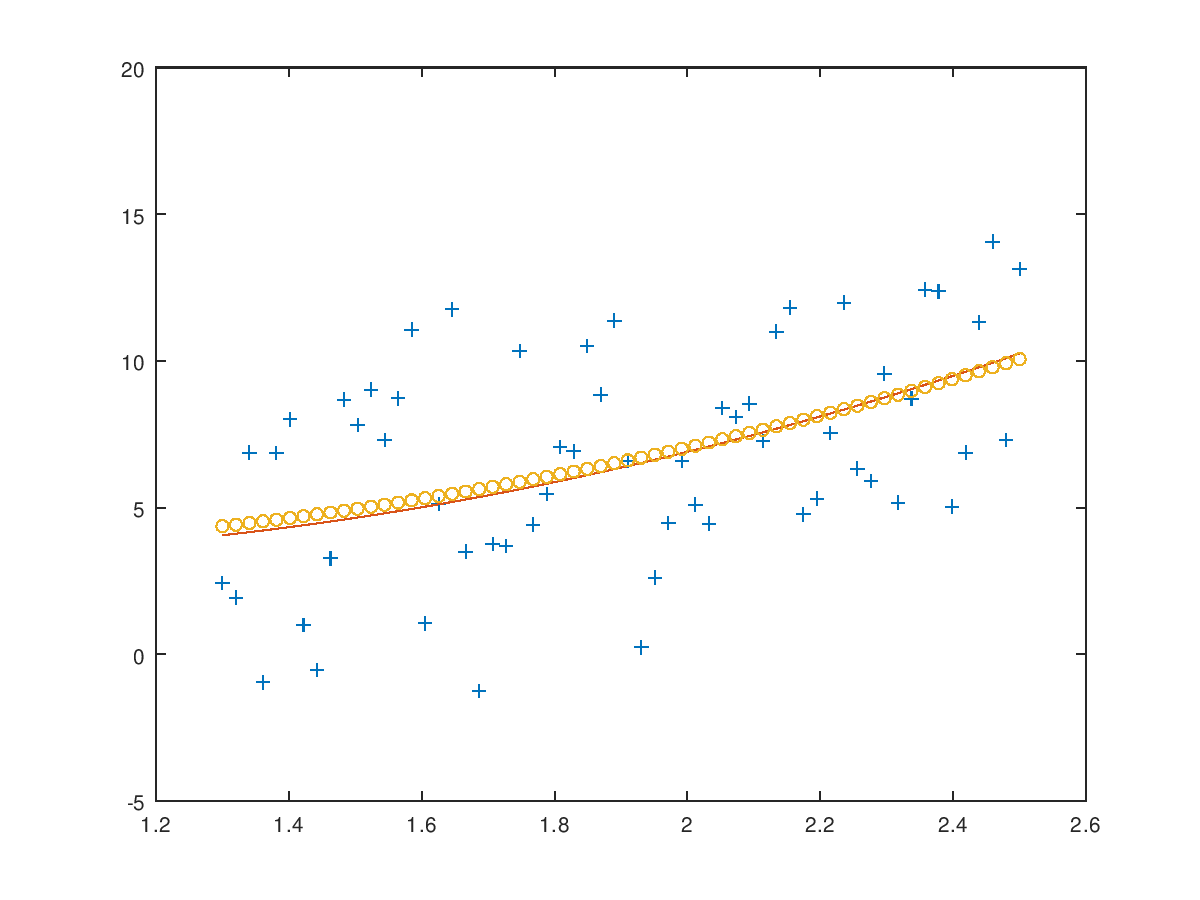
\includegraphics[scale=0.9]{g1.png}
\subsection{Линейная функция}
  \lstinputlisting{out2.txt}
  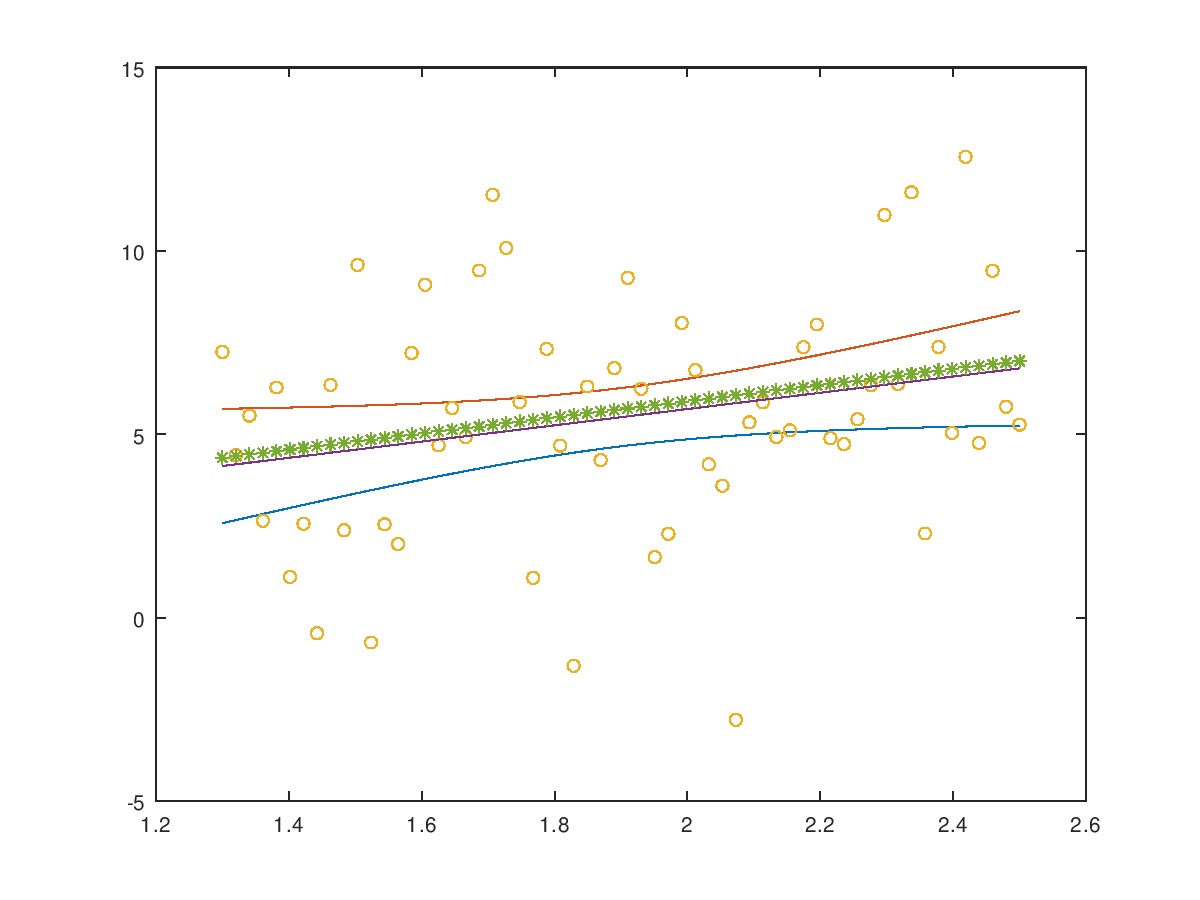
\includegraphics[scale=0.9]{g2.png}
\section{Вывод}
  Для обеих функций:
  \begin{itemize}
    \item Полученная в результате интерполяции функция хорошо приближается исходной.
    \item Посчитанный уровень шумов близок к теоретическому.
    \item Вектор несвязок практически ортогонален вектору значений зашумленной функии.
  \end{itemize}
  А также график линейной функций с посчитанными коэффициентами попадает в доверительный интервал.
\end{quote}
\end{document}
